\chapter{\IfLanguageName{dutch}{Literatuurstudie}{Literature study}}%
\label{ch:literatuurstudie}

% Tip: Begin elk hoofdstuk met een paragraaf inleiding die beschrijft hoe
% dit hoofdstuk past binnen het geheel van de bachelorproef. Geef in het
% bijzonder aan wat de link is met het vorige en volgende hoofdstuk.

% Pas na deze inleidende paragraaf komt de eerste sectiehoofding.

% Dit hoofdstuk bevat je literatuurstudie. De inhoud gaat verder op de inleiding, maar zal het onderwerp van de bachelorproef *diepgaand* uitspitten. De bedoeling is dat de lezer na lezing van dit hoofdstuk helemaal op de hoogte is van de huidige stand van zaken (state-of-the-art) in het onderzoeksdomein. Iemand die niet vertrouwd is met het onderwerp, weet nu voldoende om de rest van het verhaal te kunnen volgen, zonder dat die er nog andere informatie moet over opzoeken \autocite{Pollefliet2011}.

% Je verwijst bij elke bewering die je doet, vakterm die je introduceert, enz.\ naar je bronnen. In \LaTeX{} kan dat met het commando \texttt{$\backslash${textcite\{\}}} of \texttt{$\backslash${autocite\{\}}}. Als argument van het commando geef je de ``sleutel'' van een ``record'' in een bibliografische databank in het Bib\LaTeX{}-formaat (een tekstbestand). Als je expliciet naar de auteur verwijst in de zin (narratieve referentie), gebruik je \texttt{$\backslash${}textcite\{\}}. Soms is de auteursnaam niet expliciet een onderdeel van de zin, dan gebruik je \texttt{$\backslash${}autocite\{\}} (referentie tussen haakjes). Dit gebruik je bv.~bij een citaat, of om in het bijschrift van een overgenomen afbeelding, broncode, tabel, enz. te verwijzen naar de bron. In de volgende paragraaf een voorbeeld van elk.

% \textcite{Knuth1998} schreef een van de standaardwerken over sorteer- en zoekalgoritmen. Experten zijn het erover eens dat cloud computing een interessante opportuniteit vormen, zowel voor gebruikers als voor dienstverleners op vlak van informatietechnologie~\autocite{Creeger2009}.

% Let er ook op: het \texttt{cite}-commando voor de punt, dus binnen de zin. Je verwijst meteen naar een bron in de eerste zin die erop gebaseerd is, dus niet pas op het einde van een paragraaf.

% \begin{figure}
%   \centering
%   
\includegraphics[width=0.8\textwidth]{grail.jpg}
%   \caption[Voorbeeld figuur.]{\label{fig:grail}Voorbeeld van invoegen van een figuur. Zorg altijd voor een uitgebreid bijschrift dat de figuur volledig beschrijft zonder in de tekst te moeten gaan zoeken. Vergeet ook je bronvermelding niet!}
% \end{figure}

% \begin{listing}
%   \begin{minted}{python}
%     import pandas as pd
%     import seaborn as sns

%     penguins = sns.load_dataset('penguins')
%     sns.relplot(data=penguins, x="flipper_length_mm", y="bill_length_mm", hue="species")
%   \end{minted}
%   \caption[Voorbeeld codefragment]{Voorbeeld van het invoegen van een codefragment.}
% \end{listing}

% \lipsum[7-20]

% \begin{table}
%   \centering
%   \begin{tabular}{lcr}
%     \toprule
%     \textbf{Kolom 1} & \textbf{Kolom 2} & \textbf{Kolom 3} \\
%     $\alpha$         & $\beta$          & $\gamma$         \\
%     \midrule
%     A                & 10.230           & a                \\
%     B                & 45.678           & b                \\
%     C                & 99.987           & c                \\
%     \bottomrule
%   \end{tabular}
%   \caption[Voorbeeld tabel]{\label{tab:example}Voorbeeld van een tabel.}
% \end{table}

Als modern IT-bedrijf is het belangrijk om de veiligheid van data te garanderen als ook snelle en betrouwbare toegang tot applicaties en diensten te bieden. De opkomst van hybride cloudinfrastructuren en remote werken heeft de noodzaak voor een robuuste beveiligingsarchitectuur vergroot. Dit hoofdstuk onderzoekt de concepten van Secure Access Service Edge (SASE), Zero Trust, SD-WAN en hoe deze kunnen worden toegepast.

\section{Wat is SASE?}
Secure Access Service Edge (SASE) is een cloud-gebaseerd beveiligingsmodel dat netwerk- en beveiligingsfuncties combineert in één geïntegreerd platform. Deze technologie is ontstaan als antwoord op de toenemende complexiteit van moderne IT-infrastructuren, waarbij bedrijven steeds meer vertrouwen op cloud-diensten en verspreide werkplekken.

\vspace{2ex}

SASE biedt een oplossing die traditionele netwerkmuren doorbreekt door beveiligde toegang te verlenen aan gebruikers, ongeacht hun locatie of het apparaat dat ze gebruiken~\autocite{KPN2023}.

\vspace{2ex}

SASE is een relatief nieuw framework dat netwerk- en beveiligingsfuncties samenvoegt in één cloudgebaseerd servicemodel. Dit wordt steeds belangrijker, vooral omdat gebruikers en data nu vaak buiten het traditionele bedrijfsnetwerk werken. 

\vspace{2ex}

SASE combineert SD-WAN (Software-Defined Wide Area Networking) technologie voor netwerkoptimalisatie met cloudgebaseerde beveiligingsfuncties, waaronder Zero Trust Network Access (ZTNA), Cloud Access Security Brokers (CASB) en Firewall-as-a-Service (FWaaS)~\autocite{ZPE2025}.

\section{Vergelijkings Analyse}
De opkomst van Secure Access Service Edge (SASE) als antwoord op de beveiligings- en connectiviteitsuitdagingen van vandaag de dag brengt een kritieke vraagstelling met zich mee: hoe selecteert een software agency het optimale platform dat zowel technologische als bedrijfsmatige schaalbaarheid waarborgt? 

\vspace{2ex}

Deze vergelijkende analyse onderzoekt 3 SASE-oplossingen (Netskope, Zscaler en Palo Alto) aan de hand van zeven kerncriteria die essentieel zijn voor succesvolle adoptie in dynamische ontwikkelomgevingen.

\subsection{Criteria}

Bij de evaluatie van SASE-oplossingen zijn volgende kerncriteria essentieel:
\begin{itemize}
  \item \textbf{Architecturale Convergentie}: De SASE-oplossing moet gebouwd zijn op een unified, single-vendor architectuur die alle netwerk- en beveiligingscomponenten integreert in één besturingssysteem~\autocite{Taylor-2023}. 
  Dit elimineert de noodzaak voor meerdere producten en zorgt voor naadloze integratie tussen SD-WAN, routing, encryptie en security capabilities~\autocite{Taylor-2023}~\autocite{Anderson-2023}. De oplossing moet daarnaast compatibel zijn met bestaande security- en netwerkinfrastructuur~\autocite{Taylor-2023}.
  \item \textbf{Gecentraliseerd Policy Management met Gedistribueerde Enforcement}: Gecentraliseerde policy configuration en management gecombineerd met gedistribueerde security enforcement via Points of Presence (PoPs)~\autocite{Taylor-2023}. IT-teams moeten consistent bedrijfsbeleid kunnen toepassen op alle locaties terwijl beleidsafhandeling flexibel kan worden aangepast~\autocite{Anderson-2023}. Deze benadering waarborgt uniforme security governance ongeacht gebruikerslocatie.
  \item \textbf{Uitgebreide Analytics en Real-time Zichtbaarheid}: Een analytics engine die volledige zichtbaarheid biedt voor alle componenten van het SASE-ecosysteem, inclusief work-from-anywhere werknemers~\autocite{Anderson-2023}. De oplossing moet duidelijke analytics leveren voor gebruikerservaring, activiteit, netwerkverkeer en security events~\autocite{Taylor-2023}. Real-time insights in netwerkprestaties, gebruikersgedrag en compliance posture zijn essentieel voor effectieve IT-operaties~\autocite{Taylor-2023}.
  \item \textbf{Geïntegreerde Advanced Security Stack}: Een robuuste IDS/IPS gekoppeld aan een advanced Firewall as a Service (Next Generation Firewall) met uitgebreide classificatie- en detectiecapaciteiten~\autocite{Taylor-2023}. De security functies moeten geïntegreerd worden geleverd als één oplossing en real-time threat detection mogelijk maken~\autocite{Anderson-2023}. Multi-layered beveiligingscontroles moeten naadloos samenwerken binnen de unified architectuur.
  \item \textbf{Dynamische Schaalbaarheid met Flexibele Licentiemodellen}: De oplossing moet geleverd worden als Software as a Service (SaaS) met elastische schaalbaarheid die dynamisch aanpast aan klantbehoeften~\autocite{Taylor-2023}. Licensing moet eenvoudige schaalmogelijkheden bieden om pieken in vraag te accommoderen~\autocite{Anderson-2023}. Elasticiteit is vereist voor zowel data plane als control en management planes~\autocite{Taylor-2023}.
  \item \textbf{End-to-End Gebruikerservaring}: De oplossing moet een naadloze, gebruiksvriendelijke, consistente ervaring bieden over verschillende apparaten, applicaties en locaties~\autocite{Anderson-2023}. Rapid turn-up capabilities moeten IT-teams in staat stellen beleid snel te provisionen voor honderden of duizenden gebruikers~\autocite{Anderson-2023}.
\end{itemize}

\subsection{Vergelijking}
De onderstaande vergelijking positioneert 3 toonaangevende SASE-leveranciers volgens Gartner en evalueert deze op basis van hun architecturale benadering, technische sterke punten en operationele beperkingen. Deze methodiek zorgt voor een objectieve beoordeling die verder gaat dan marketingclaims en zich richt op bewezen implementatie-ervaring binnen enterprise-omgevingen~\autocite{Gartner2025}.

\subsubsection{Netskope}
\textbf{Categorie:} Leader

\textbf{Architectuur:}  Volledig geïntegreerde SSE gecombineerd met SD-WAN-functionaliteiten via het eigen NewEdge-netwerk.

\textbf{Sterktes}
\begin{itemize}
    \item Bewezen technische superioriteit met meer dan 3.000 vooraf geconfigureerde DLP-regels die dekking bieden voor internationale compliance-vereisten en industriespecifieke regelgeving.
    \item Gegarandeerde netwerkprestaties met een 50ms latency SLA ondersteund door een uitgebreid globaal netwerk van meer dan 71 strategisch geplaatste Points of Presence.
    \item Geavanceerde data-gerichte Zero Trust benadering die zich richt op real-time data classificatie en contextbewuste toegangscontroles.
\end{itemize}

\textbf{Beperkingen}
\begin{itemize}
    \item Primaire focus ligt uitsluitend op enterprise-markt, waardoor de oplossing minder geschikt kan zijn voor kleinere organisaties met beperkte budgetten.
    \item Relatief trage implementatie van nieuwe features en functionaliteiten vergeleken met concurrenten in de markt.
    \item Beperkte taalondersteuning met hoofdzakelijk Engelstalige interface, wat adoptie kan belemmeren in niet-Engelssprekende organisaties.
\end{itemize}
~\autocite{Gartner2025}

\subsubsection{Zscaler}
\textbf{Categorie:} Leader

\textbf{Architectuur:} Cloud-native architectuur met gescheiden modules voor internet access (ZIA) en private access (ZPA) die via een central management console worden beheerd.

\textbf{Sterktes}
\begin{itemize}
    \item Marktleidende positie met de sterkste marketingpositie en brandherkenning binnen de SASE markt, ondersteund door uitgebreide partnerschappen.
    \item Transparant en vereenvoudigd prijsmodel dat voorspelbare kosten biedt en eenvoudige budgetplanning mogelijk maakt voor organisaties.
    \item Bewezen track record met een hoog adoptiecijfer en uitgebreide klantenbasis over verschillende industrieën en organisaties.
\end{itemize}

\textbf{Beperkingen}
\begin{itemize}
    \item Technische scheiding tussen ZIA en ZPA-modules kan leiden tot complexere configuratie en potentiële integratie-uitdagingen.
    \item Relatief hoge totale eigendomskosten, vooral bij volledige feature-sets, wat budgetbeperkingen kan creëren voor kost-gevoelige organisaties.
\end{itemize}
~\autocite{Gartner2025}

\subsubsection{Palo Alto}
\textbf{Categorie:} Leader

\textbf{Architectuur:} Volledig geïntegreerde Firewall-as-a-Service (FWaaS) gecombineerd met SD-WAN-functionaliteiten binnen het Prisma SASE-platform.
\textbf{Sterktes}
\begin{itemize}
    \item Geavanceerde AI-gestuurde dreigingsdetectie en preventie.
    \item Naadloze integratie met bestaande on-premises Palo Alto firewalls, waardoor organisaties hun huidige investeringen kunnen behouden en geleidelijk kunnen migreren.
    \item Substantiële R\&D-investering, wat resulteert in continue innovatie en cutting edge security functionaliteiten.
\end{itemize}

\textbf{Beperkingen}
\begin{itemize}
    \item Complexe en moeilijk voorspelbare prijsstructuur met verschillende licentiemodellen die budgetplanning kan bemoeilijken.
    \item Beperkte taalondersteuning en lokalisatie, kan adoptie belemmeren in diverse internationale organisaties.
    \item Relatief smalle use cases vergeleken met concurrenten, met focus op specifieke security-scenario's in plaats van brede SASE-implementaties.
\end{itemize}
~\autocite{Gartner2025}

\vspace{2ex}

Netskope, Zscaler en Palo Alto Networks zijn de drie marktleiders met verschillende sterke punten. Netskope biedt de beste technische specificaties met 3.000+ DLP-regels en een 50ms prestatie-SLA via één geïntegreerd platform. Zscaler heeft het grootste marktaandeel en sterke merkherkenning, maar hun ZIA en ZPA modules werken gescheiden wat operationeel complex is.

Palo Alto Networks excelleert in AI-gestuurde security en integreert goed met bestaande firewalls, maar hun prijsmodel is complex en duur. Voor software agencies is Netskope de beste keuze omdat het technische diepgang combineert met operationele eenvoud. Waar Zscaler fragmentatie introduceert en Palo Alto kostbaar is, levert Netskope een complete oplossing met garanties die essentieel zijn voor ontwikkelomgevingen.

\section{Het gekozen platform, Netskope}
Netskope is gekozen als het platform voor de implementatie van de SASE-architectuur. Netskope onderscheidt zich door zijn geïntegreerde benadering van netwerk- en beveiligingsdiensten via het Netskope One Platform. 

\vspace{2ex}

De geïntegreerde architectuur van Netskope elimineert de tool-fragmentatie die bij concurrenten voorkomt, terwijl de expliciete prestatie-SLA's zekerheid bieden voor kritieke applicaties. Dit maakt Netskope de logische keuze voor het proof of concept binnen de hybride cloudinfrastructuur van een software agency.

\vspace{2ex}

Dit platform combineert geavanceerde technologieën zoals de Zero Trust Engine, NewEdge-netwerk en uitgebreide DLP-functionaliteiten om zowel beveiliging als connectiviteit te optimaliseren~\autocite{Netskope2025-1}.

\vspace{2ex}

In tegenstelling tot andere SASE-leveranciers biedt Netskope een volledig geïntegreerd platform zonder afhankelijkheid van meerdere leveranciers of gescheiden oplossingen. Dit vermindert operationele complexiteit, verbetert de gebruikerservaring en zorgt voor consistente beleidsimplementatie over alle netwerk- en beveiligingslagen heen~\autocite{Netskope2025-1}.

\subsection{Kernpijlers}
De SASE-architectuur van Netskope rust op vier essentiële kernpijlers die samen een omvattend beveiligings-framework vormen, specifiek afgestemd op de uitdagingen van moderne hybride cloudomgevingen:

\begin{itemize}
  \item \textbf{Zero Trust Engine}: Deze kerncomponent biedt contextbewuste beveiliging door risico's in real-time te analyseren op basis van meer dan 50 variabelen, zoals gebruikersgedrag, apparaatprofielen en applicatiecontext. Dit stelt organisaties in staat om adaptieve toegangscontrole toe te passen en risico's proactief te beheren~\autocite{Netskope2025-2}.
  \item \textbf{NewEdge-netwerk}: Het grootste private cloudnetwerk ter wereld biedt lage latentie en optimale prestaties voor SaaS-applicaties, webverkeer en privétoepassingen. Dit netwerk maakt gebruik van uitgebreide peeringrelaties om snelle toegang te garanderen zonder prestatieverlies~\autocite{Netskope2025-1}.
  \item \textbf{DLP}: Netskope biedt uitgebreide databescherming door middel van AI-gestuurde detectie en classificatie van gevoelige gegevens over netwerken, endpoints en cloudomgevingen~\autocite{Netskope2025-1}.
  \item \textbf{Geïntegreerde SD-WAN}: Voor het optimaliseren van netwerken op locatie en het verbinden van filialen met de cloud via veilige verbindingen~\autocite{Netskope2025-1}.
\end{itemize}

\vspace{2ex}

Met deze geïntegreerde aanpak biedt Netskope een robuuste oplossing voor bedrijven die willen overstappen naar een modern SASE-model. Het platform combineert geavanceerde technologieën met schaalbare architectuur, wat essentieel is voor het waarborgen van veiligheid, prestaties en compliance.

\section{Zero Trust}
Zero Trust is een model dat gebaseerd is op de stelling dat geen enkel apparaat, gebruiker of systeem automatisch te vertrouwen is, zelfs niet als deze zich binnen het netwerk bevinden~\autocite{Netskope2024}.

\vspace{2ex}

De nadruk ligt op het continu verifiëren van gebruikersidentiteit, het beperken van toegang tot strikt noodzakelijke bronnen (least privileged access), en het monitoren van netwerkactiviteiten om verdachte handelingen snel te identificeren en aan te pakken.

\vspace{2ex}

Volgens Microsoft is de kern van het Zero Trust-model gebaseerd op vier belangrijke principes: altijd verifiëren, nooit vertrouwen, minimaal toegang verlenen en schade beperken bij inbreuk. Dit houdt in dat de toegang tot systemen of data niet alleen wordt beperkt op basis van de locatie van de gebruiker of het apparaat, maar altijd afhangt van de identiteit, rol en andere specifieke toegangsbeperkingen~\autocite{Microsoft2024}. 

\vspace{2ex}

Kaspersky benadrukt het belang van de technologieën die Zero Trust mogelijk maken, zoals multi-factor authenticatie (MFA), versleuteling van communicatie en geavanceerde netwerkmonitoringtool. ``De omslag naar hybride werken en de toename van het aantal cyberbedreigingen die ook nog eens steeds complexer worden, betekent dat cyberweerbaarheid voor veel organisaties de hoogste prioriteit heeft.''~\autocite{Kaspersky2024}. Cyberweerbaarheid houdt in dat we onze focus moeten verleggen van preventie van cyberaanvallen naar de acceptatie dat dit soort aanvallen tegenwoordig onvermijdelijk zijn en we ervoor moeten zorgen dat organisaties zo goed mogelijk zijn voorbereid op eventuele aanvallen en deze snel en effectief kunnen herstellen. Zero Trust speelt hier een belangrijke rol in~\autocite{Kaspersky2024}.

\vspace{2ex}

NIST definieert Zero Trust Architecture (ZTA) als een volledig cybersecurity-plan dat nooit impliciet vertrouwen verleent, maar continu evalueert. ZTA richt zich op het beschermen van alle resources van gegevensbronnen tot netwerkapparatuur door strikte authenticatie, autorisatie en encryptie toe te passen bij elk toegangsverzoek~\autocite{NIST2020}.

\vspace{2ex}

Dit onderzoek naar Zero Trust Network Architecture (ZTNA) biedt waardevolle inzichten in de evolutie van netwerkbeveiliging als directe reactie op de uitdagingen die ontstonden door de COVID-19 pandemie. De massale overgang naar remote werken dwong organisaties om hun traditionele beveiligingsmodellen fundamenteel te heroverwegen, waarbij de beperkingen van het "castle-and-moat" concept duidelijk naar voren kwamen. Het castle-and-moat concept is een traditioneel netwerkbeveiligingsmodel dat zijn naam ontleent aan de architectuur van middeleeuwse kastelen. Net zoals een kasteel werd beschermd door een gracht (moat) en stevige muren, baseert dit beveiligingsmodel zich op het principe van perimeterbescherming rond het bedrijfsnetwerk~\autocite{Deshpande-2021}. 

\vspace{2ex}

Deze traditionele benadering, waarbij eenmaal toegang tot het netwerk was verkregen via de firewall, gebruikers relatief vrij konden navigeren door het gehele netwerk, bleek ontoereikend voor een verspreide werkplek waar werknemers vanuit verschillende locaties toegang nodig hadden tot bedrijfsbronnen~\autocite{Deshpande-2021}.

\subsection{Kernprincipes van Zero Trust}
\label{sec:Kernprincipes van Zero Trust}
Zeven fundamentele principes vormen de basis van NIST’s Zero Trust-architectuur~\autocite{NIST2020}:  

\begin{itemize}
  \item \textbf{Alle resources als entiteiten beschouwen}: Zowel kleine apparaten als complexe systemen worden behandeld als beveiligingsobjecten die specifieke controles vereisen.  
  \item \textbf{Beveiligde communicatie ongeacht locatie}: Netwerksegmentatie biedt geen automatisch vertrouwen, interne apparaten moeten aan dezelfde beveiligingseisen voldoen als externe.  
  \item \textbf{Toegang per sessie}: Vertrouwen in de aanvrager wordt geëvalueerd vóór toegang wordt verleend, met minimale rechten om een taak uit te voeren.  
  \item \textbf{Dynamisch beleid}: Toegang wordt gebaseerd op contextuele factoren zoals identiteit, apparaatstatus, gedragsanalyse en omgevingsvariabelen.  
  \item \textbf{Continu monitoring van integriteit}: Geen enkel apparaat wordt blind vertrouwd; beveiligingsstatus wordt bij elke aanvraag gecontroleerd.  
  \item \textbf{Dynamische authenticatie en autorisatie}: Validatie gebeurt tijdens de sessie, met mogelijkheid tot herauthenticatie bij ongewoon gedrag.  
  \item \textbf{Maximale informatieverzameling}: Zichtbaarheid over assets, netwerkverkeer en gebruikersactiviteiten dient als input voor risico-evaluatie en beleidsaanpassing.  
\end{itemize}

\subsection{Implementatiestrategieën}
NIST raadt drie benaderingen aan voor migratie naar ZTA~\autocite{NIST2020}:

\begin{itemize}
  \item \textbf{Versterkt identiteitsbeheer}: Identiteit als kerncomponent voor toegangsbeslissingen, gekoppeld aan multi-factor authenticatie en risicoscoring.  
  \item \textbf{Micro-segmentatie}: Resources isoleren in unieke netwerksegmenten, beschermd door PEPs, om laterale bewegingen te beperken.  
  \item \textbf{Netwerkinfrastructuur en Software Defined Perimeters}: Gebruik van SD-WAN en cloudgebaseerde netwerkbeveiliging om Zero Trust-principes toe te passen.  
\end{itemize}

\subsection{Migratieproces}
Organisaties moeten een gefaseerde aanpak volgen~\autocite{NIST2020}:  
\begin{itemize}
  \item \textbf{Identificatie van actoren en resources}: Inventarisatie van gebruikers, apparaten en kritieke assets.  
  \item \textbf{Beleiddefinitie}: Ontwikkeling van dynamische regels gebaseerd op risicoprofielen en compliance-eisen.  
  \item \textbf{Implementatie en monitoring}: Geleidelijke uitrol met continue evaluatie van prestaties en aanpassing van beleid.  
\end{itemize}

\subsection{Uitdagingen en beperkingen}
ZTA reduceert risico’s maar elimineert ze niet volledig. Belangrijke bedreigingen omvatten~\autocite{NIST2020}:  
\begin{itemize}
  \item \textbf{Insiderdreigingen}: Misbruik van gecompromitteerde credentials.  
  \item \textbf{Netwerkverstoringen}: Denial-of-Service-aanvallen op PEPs.  
  \item \textbf{Beperkte zichtbaarheid}: Moeilijkheden bij het detecteren van verdachte activiteiten in gedistribueerde omgevingen.  
\end{itemize}

NIST benadrukt dat volgende elementen cruciaal zijn voor een vlotte implementatie~\autocite{NIST2020}:  
\begin{itemize}
  \item \textbf{Interoperabiliteit}: Integratie met bestaande Identity Providers en SIEM-systemen.  
  \item \textbf{Organisatorische aanpassingen}: Training van medewerkers en duidelijke incidentresponse-processen.
\end{itemize}

\subsection{Technische Implementatievarianten}
Zero Trust-architectuur manifesteert zich in verschillende technische implementaties, elk met specifieke toepassingsgebieden en voordelen. StrongDM~\autocite{StrongDM2025} identificeert drie hoofdvarianten die organisaties kunnen implementeren binnen hun beveiligingsstrategie.

\begin{itemize}
  \item \textbf{Zero Trust Network Access (ZTNA)}: functioneert als een "software-defined perimeter" die traditionele VPN-oplossingen vervangt door microsegmentatie en netwerkisolatie. Deze benadering creëert dynamische beveiligingsperimeters rond specifieke resources en gebruikers, waarbij toegang wordt verleend op basis van continue verificatie in plaats van netwerklocatie. ZTNA sluit naadloos aan bij Netskope's Policy Enforcement Points op netwerkniveau, waarbij granulaire toegangscontrole wordt toegepast zonder de complexiteit van traditionele firewall-regelsets~\autocite{StrongDM2025}.
  \item \textbf{Zero Trust Application Access (ZTAA)}: breidt Zero Trust-principes uit naar applicatieniveau, waarbij toegang wordt beperkt tot na verificatie van zowel gebruikers als apparaten. Deze implementatie is bijzonder relevant voor software agencies die werken met gevoelige klantdata en meerdere ontwikkelomgevingen. ZTAA complementeert Netskope's Application PEP door applicatie-specifieke beleidsregels toe te passen die verder gaan dan traditionele netwerkbeveiliging~\autocite{StrongDM2025}.
  \item \textbf{Zero Trust Access}: functioneert als overkoepelend model dat zowel ZTAA als ZTNA omvat, waardoor end-to-end Zero Trust wordt gerealiseerd over de gehele architectuur. Deze  benadering sluit direct aan bij SASE-principes door netwerk- en beveiligingsfuncties te convergeren in één unified platform~\autocite{StrongDM2025}.
\end{itemize}

\vspace{2ex}

\subsection{Multi-layered Beveiligingsbenadering voor Hybride Cloudomgevingen}
De implementatie van Zero Trust vereist een meerlagige aanpak. Deze integreert netwerkssegmentatie, Layer 7 threat prevention, granulaire gebruikerstoegangscontrole, uitgebreide beveiigingsmonitoring en security system automation. Deze benadering is bijzonder relevant geworden door de opkomst van remote werken, bring-your-own-device (BYOD) beleid en cloudgebaseerde assets die zich buiten traditionele enterprise-netwerkgrenzen bevinden~\autocite{StrongDM2025}.

\vspace{2ex}

Voor software agencies betekent dit dat Zero Trust niet alleen technologische verandering vereist, maar ook organisatorische aanpassingen in werkprocessen en gebruikersgedrag. De convergentie van deze beveiligingslagen binnen een SASE-architectuur zoals Netskope zorgt ervoor dat beveiligingsbeleid consistent wordt toegepast ongeacht waar ontwikkelaars, designers en projectmanagers zich bevinden of welke apparaten zij gebruiken.

\section{Policy Enforcement Points}
Netskope implementeert de principes die besproken worden in sectie~\ref{sec:Kernprincipes van Zero Trust} in een gelaagde aanpak met Policy Enforcement Points (PEPs) op drie niveaus:

\begin{itemize}
  \item \textbf{Network/Resource PEP}: controleert netwerktoegang en basiscommunicatie
  \item \textbf{Application PEP}: beheert toegang tot specifieke applicaties en workloads
  \item \textbf{Data PEP}: zorgt voor databescherming en compliance
\end{itemize}

Figuur~\ref{fig:Netskope-PEP} toont een uitgebreid Zero Trust architectuurmodel dat drie hoofdcomponenten naadloos integreert: identiteits- en toegangsbeheer, resourcebescherming en controlefuncties. 

\vspace{2ex}

Aan de linkerzijde begint het proces met twee mogelijke entiteiten (niet-persoons- of gebruikersentiteiten) die authenticatie en autorisatie ondergaan, waarbij device-compliance, locatie, toegangstype en -methode worden geëvalueerd in samenwerking met een gefedereerde identiteitsservice (IDP)~\autocite{Netskope2024}. 

\vspace{2ex}

Het middelste gedeelte illustreert de gelaagde resourcebeveiliging met drie opeenvolgende autorisatieniveaus: resource-, applicatie- en datautorisatie, elk met hun eigen Policy Enforcement Point (PEP) en specifieke beveiligingscapaciteiten zoals microsegmentatie, app-instancing en datarechten management~\autocite{Netskope2024}. 

\vspace{2ex}

De rechterzijde vertegenwoordigt het centrale controlesysteem dat bestaat uit een Policy Engine die wordt ondersteund door SOAR (Security Orchestration, Automation and Response), analytische vertrouwensscoring, SIEM (Security Information and Event Management) en event logging~\autocite{Netskope2024}. 

\vspace{2ex}

De blauwe pijlen tonen hoe de Policy Engine directe controle uitoefent over alle PEPs. De stippellijnen illustreren daarentegen de feedback-loops die essentieel zijn voor een dynamisch Zero Trust beveiligingsmodel. Dit model wordt voortdurend bijgesteld op basis van actuele dreigingsinformatie en gebruikersgedrag. Deze aanpak is cruciaal voor een effectieve SASE-implementatie in hybride cloudomgevingen, zoals die van een software agency bedrijf.~\autocite{Netskope2024}.
\begin{figure}[H]
  \centering
  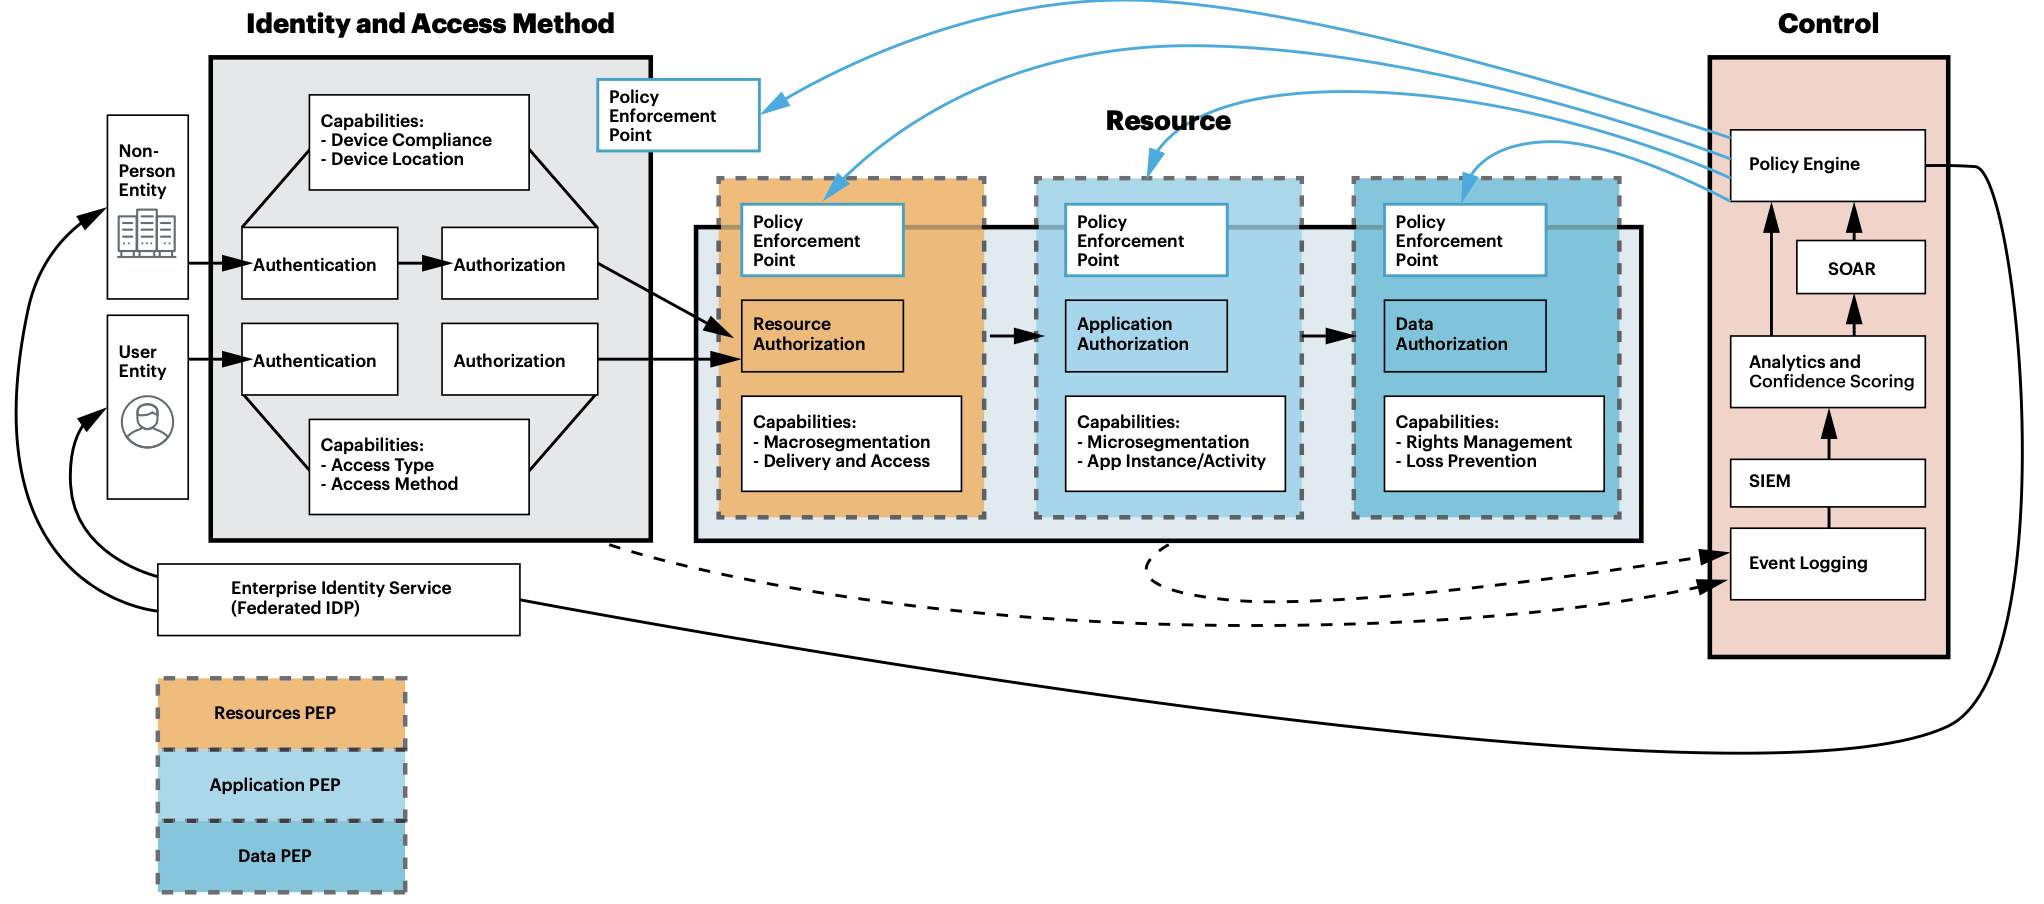
\includegraphics[width=\textwidth]{Netskope-PEP.png}
  \caption[Netskope Policy Enforcement Points (PEPs)]{Policy Enforcement Points (PEPs) in Netskope's Zero Trust Security Service Edge (SSE) platform~\autocite{Netskope2024}}
  \label{fig:Netskope-PEP}
\end{figure}


Netskope's platform integreert deze technologieën in een uitgebreid security framework dat onder andere bestaat uit:

\begin{itemize}
  \item Device en user authenticatie via een client certificaat infrastructuur
  \item Data Loss Prevention (DLP) met meer dan 3000 data identifiers en 1400 bestandstypes
  \item Software Defined WAN (SD-WAN) voor het samenvoegen van netwerken op site's met de cloud.
  \item Real-time threat protection met meer dan 40 threat intelligence feeds
\end{itemize}

Figuur~\ref{fig:Netskope-user-and-device} beschrijft het uitgebreide authenticatie- en validatieproces voor gebruikers en apparaten binnen de Netskope Zero Trust implementatie. 

\vspace{2ex}

De workflow begint wanneer een gebruiker toegang vraagt. Eerst wordt de apparaatconfiguratie gevalideerd en de locatie bepaald via on-premise detectie. Vervolgens volgt één van drie authenticatiepaden: Domain Multi-User, Domain Single User of SAML/SSO. Elk pad heeft specifieke verificatiestappen. Centrale elementen in dit proces zijn de UPN (User Principal Name) extractie voor identificatie, LDAP-gebruikersverificatie, groepsautorisatie via LDAP of SAML, en certificaatvalidatie. De Netskope Control Plane coördineert de verschillende autorisatieprocessen, past beveiligingsconfiguraties toe en zorgt voor de opzet van een versleutelde tunnel voor veilige communicatie. Rechts in het diagram worden de gebruikersattributen weergegeven die aan Netskope worden verzonden, waaronder UPN, e-mail, apparaatbeheersstatus, geïnstalleerde applicaties en diverse metadata, wat bijdraagt aan een context-bewuste beveiligingsbeoordeling in een hybride cloudscenario~\autocite{Netskope2024}.
\begin{figure}[H]
  \centering
  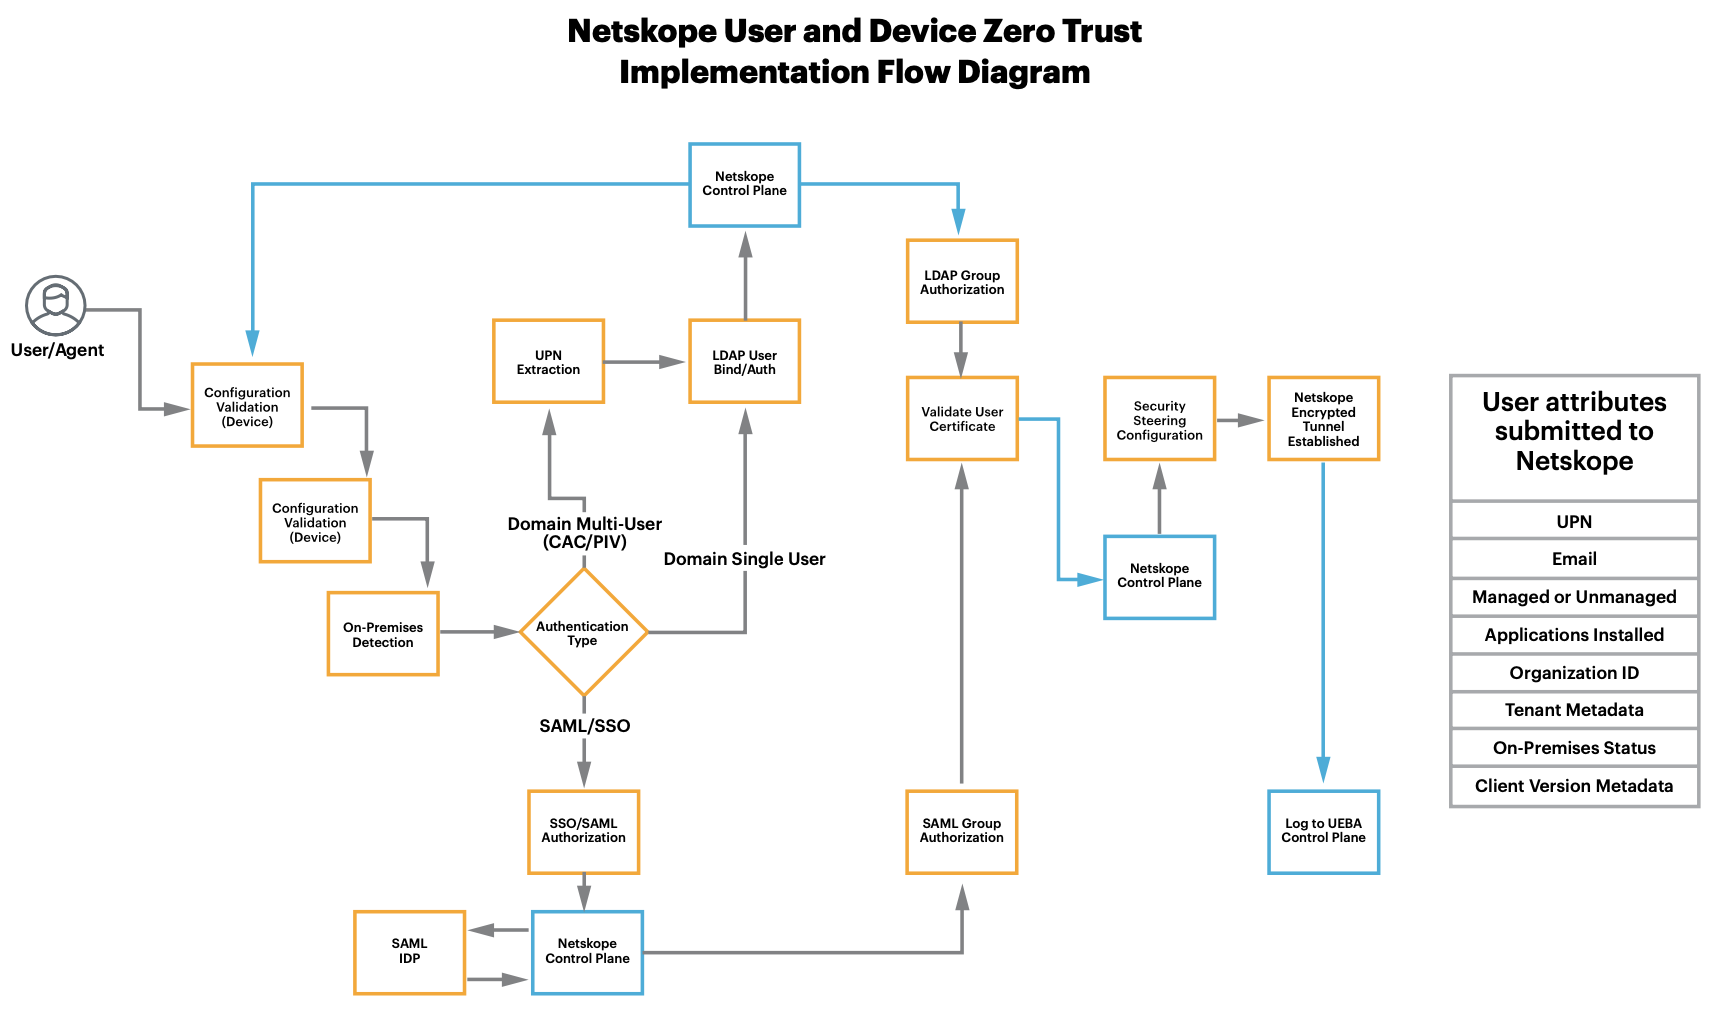
\includegraphics[width=\textwidth]{Netskope-user-and-device.png}
  \caption[Netskope Gebruiker \& Apparaat authenticatie]{Gebruiker \& Apparaat authenticatie in Netskope's Zero Trust Security Service Edge (SSE) platform~\autocite{Netskope2024}}
  \label{fig:Netskope-user-and-device}
\end{figure}

De Figuur~\ref{fig:Netskope-DLP} illustreert het Data Loss Prevention (DLP) en Digital Rights Management (DRM) implementatieproces binnen het Netskope Zero Trust raamwerk. 

\vspace{2ex}

Het proces start met een inline toegangsverzoek, dat vervolgens door meerdere analyselagen gaat, beginnend met bestandsmetadata- en contentscanning, gevolgd door compliance policy evaluatie en DLP regelprofielen. Bijzonder aan deze workflow is de parallelle toepassing van zes geavanceerde analysetechnieken: Keyword Matching, Indexed Document Matching, Exact Data Matching, OCR/Fingerprinting, Image Classifiers en Text Classifiers. De Data PEP werkt als centraal beslissingspunt dat op basis van Booleaanse logica bepaalt welke actie moet worden ondernomen. De mogelijke uitkomsten omvatten directe toegang (Allow), toegangsweigering (Block), remediëring met extra beveiligingsmaatregelen zoals multi-factor authenticatie of encryptie, of beperkte toegang met uitzonderingen. 

\vspace{2ex}

Dit gehele proces vormt een diepgaande beveiligingslaag die specifiek gericht is op databescherming en preventie van datalekken binnen het SASE-architectuurraamwerk~\autocite{Netskope2024}.
\begin{figure}[H]
  \centering
  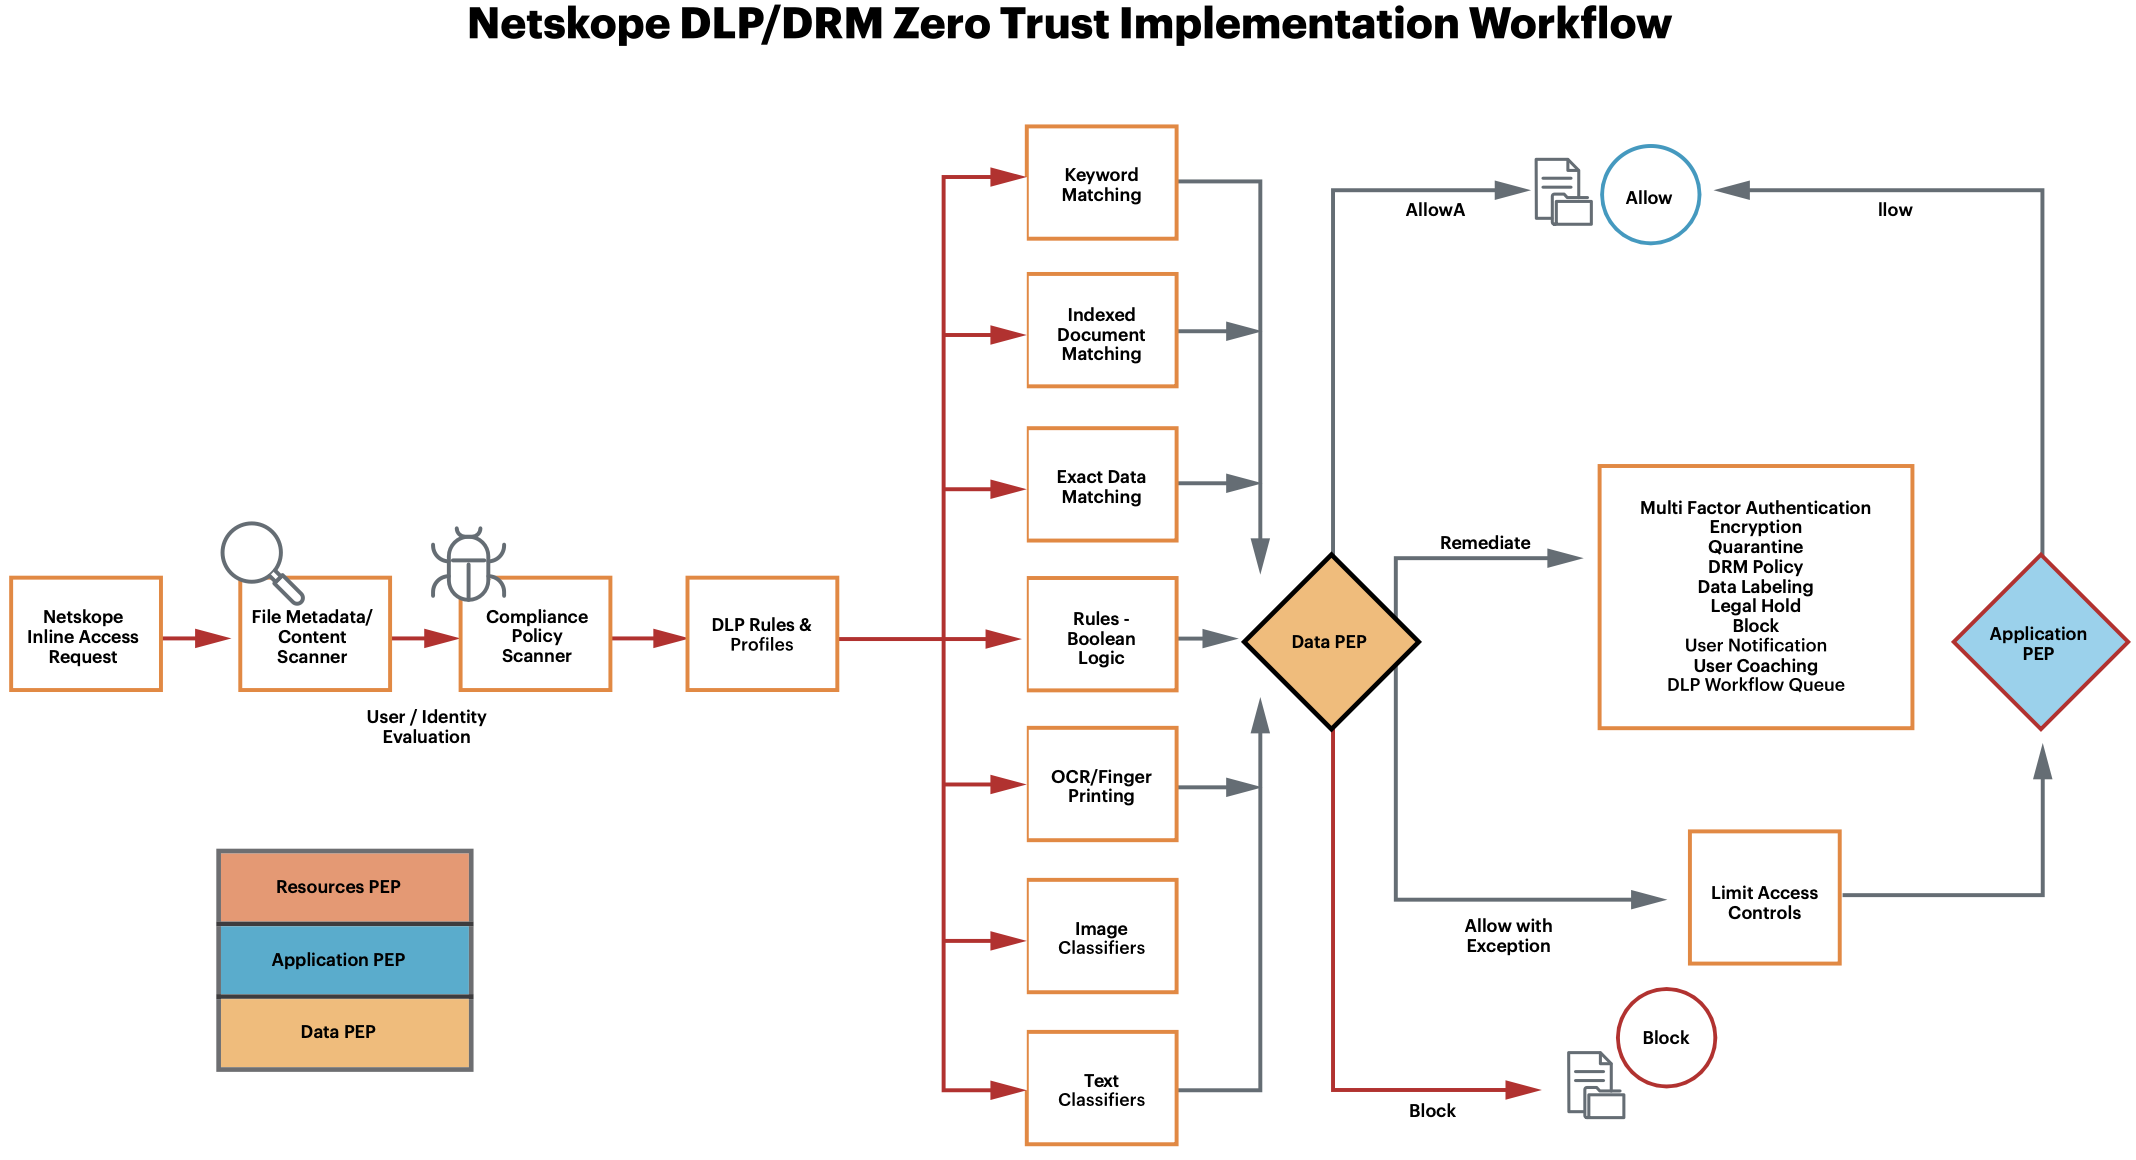
\includegraphics[width=\textwidth]{Netskope-DLP.png}
  \caption[Netskope Data Loss Prevention (DLP)]{Data Loss Prevention (DLP) in Netskope's Zero Trust Security Service Edge (SSE) platform~\autocite{Netskope2024}}
  \label{fig:Netskope-DLP}
\end{figure}

Figuur~\ref{fig:Netskope-SD-WAN} toont een gedetailleerd stroomdiagram voor de implementatie van Zero Trust principes binnen een Software-Defined Wide Area Network (SD-WAN) omgeving met Netskope. 

\vspace{2ex}

De workflow begint bij een entiteit die toegang zoekt tot een applicatie en doorloopt vervolgens verschillende beveiligingslagen. 

\vspace{2ex}

Eerst vindt device- en gebruikersverificatie plaats via het Netskope Control Plane, gevolgd door authenticatie en autorisatie. Na succesvolle authenticatie wordt de verbinding via een SD-WAN Endpoint geleid en een Port 443 Tunnel opgezet. Het cruciale beslissingspunt is de Resource PEP (Policy Enforcement Point) die evalueert of toegang moet worden verleend op basis van vooraf gedefinieerde beveiligingsregels. Bij goedkeuring wordt de verbinding via de Netskope Stitcher doorgestuurd naar de SD-WAN Publisher die de verbinding beschikbaar maakt op het oorspronkelijke protocol/poort voor de applicatie. Bij afwijzing wordt de toegang geblokkeerd, de gebruiker genotificeerd, activiteiten gelogd en risicobeoordelingen bijgewerkt~\autocite{Netskope2024}.
\begin{figure}[H]
  \centering
  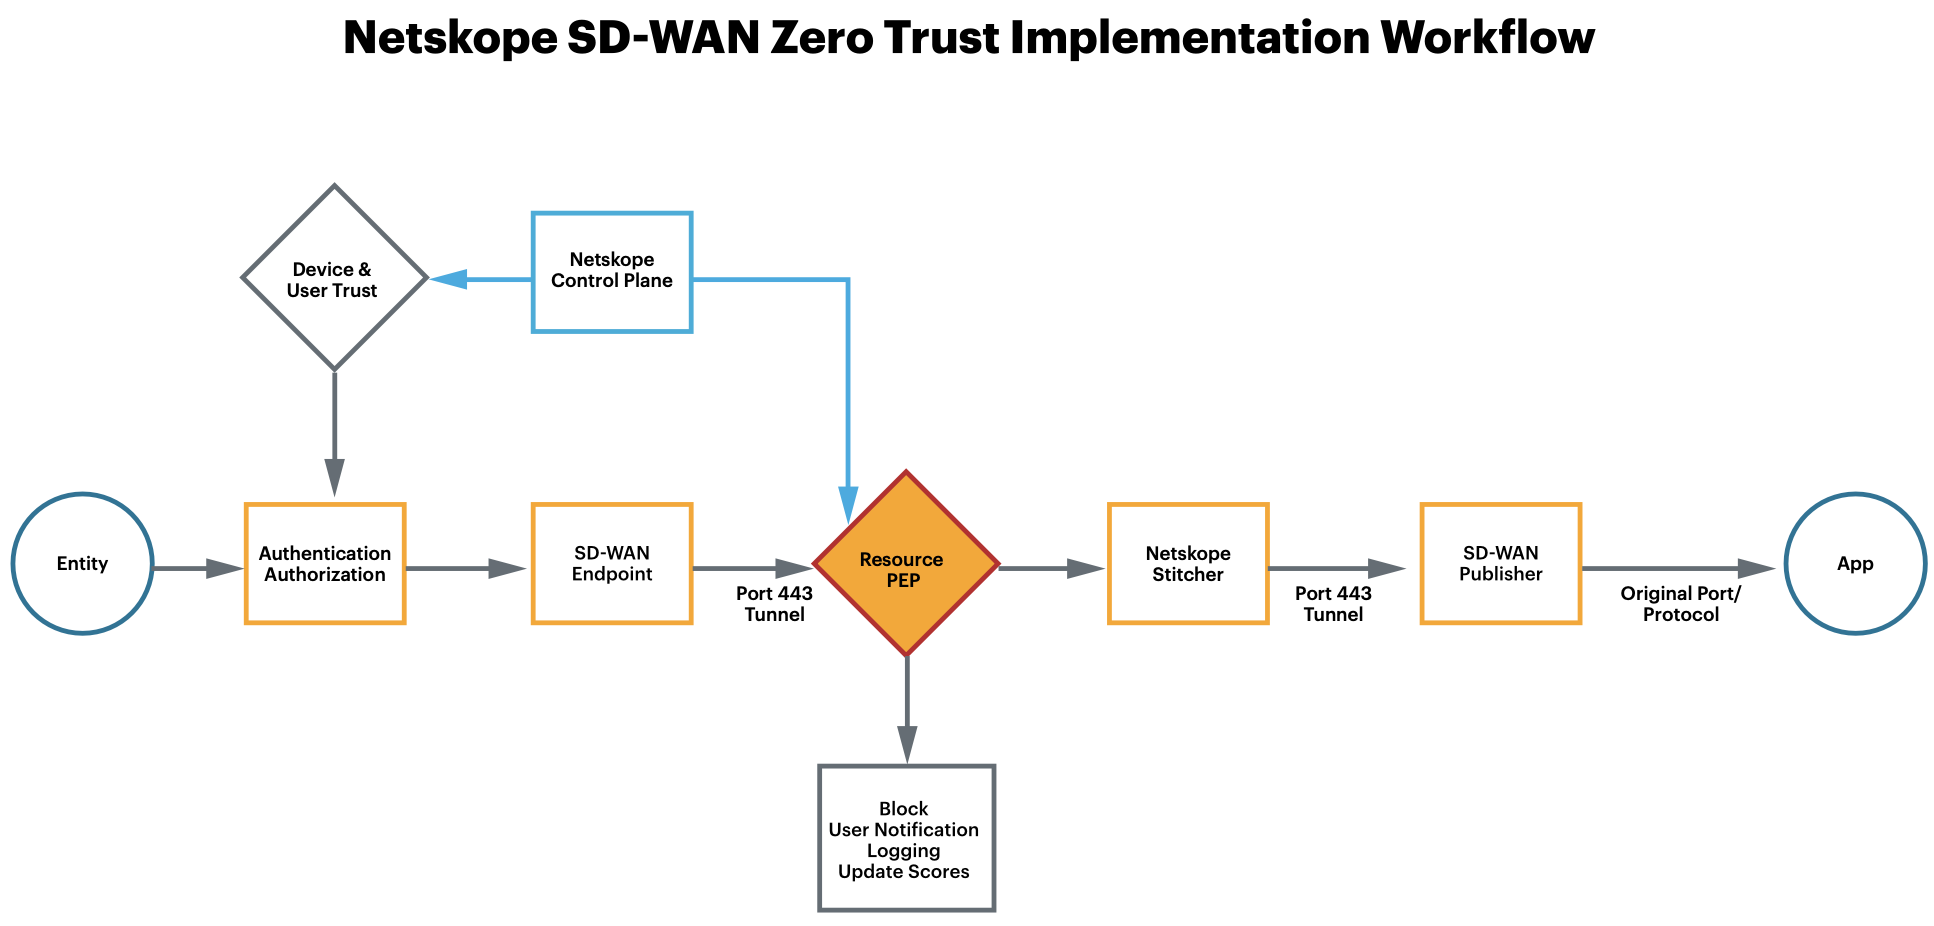
\includegraphics[width=\textwidth]{Netskope-SD-WAN.png}
  \caption[Netskope Software Defined WAN (SD-WAN)]{Software Defined WAN (SD-WAN) in Netskope's Zero Trust Security Service Edge (SSE) platform~\autocite{Netskope2024}}
  \label{fig:Netskope-SD-WAN}
\end{figure}

\vspace{2ex}

Uit onderzoek van MIT Lincoln Laboratory~\autocite{MIT2022} blijkt dat Zero Trust-architecturen bijzonder effectief zijn tegen insiderdreigingen, zoals misbruik van gecompromitteerde credentials of onbevoegde toegang door eigen medewerkers. 
Dit risico is relevant voor het onderzochte bedrijf, waar ontwikkelaars en externe partners toegang hebben tot gevoelige klantdata. 

\vspace{2ex}

MIT benadrukt dat een succesvolle Zero Trust-implementatie niet alleen technologische verandering vereist (zoals granular access control), maar ook organisatorische aanpassingen, zoals het trainen van medewerkers en het opstellen van een duidelijk beleid voor toegangsverificatie. 
Dit sluit aan bij Netskope’s focus op User \& Device workflows en gedragsanalyse, waarbij continue verificatie van gebruikers en apparaten centraal staat. 
Tegelijkertijd waarschuwt MIT voor de complexiteit van hybride implementaties, waarbij on-premises systemen en clouddiensten geïntegreerd moeten worden, een uitdaging die het bedrijf direct ondervindt en waar Netskope’s SSE-platform een antwoord op biedt~\autocite{MIT2022}.

\vspace{2ex}

Netskope biedt hiervoor een gestructureerde aanpak met specifieke operationele workflows:
\begin{itemize}
  \item \textbf{User/Device workflow}: voor initiële authenticatie en continue validatie
  \item \textbf{Network/Resource workflow}: voor toegangscontrole en segmentatie
  \item \textbf{Data Protection workflow}: voor databescherming en compliance
\end{itemize}

\vspace{2ex}

Het onderzoek van ACM~\autocite{ACM2021} levert een belangrijke bijdrage aan ons begrip van de veranderende aard van cybersecurity in een post-pandemische wereld. Hun studie bevestigt dat traditionele perimeterbescherming fundamenteel is uitgedaagd door de verschuiving naar gedistribueerde werkomgevingen.
De auteurs besluiten dat organisaties moeten evolueren van een perimeter-gebaseerd beveiligingsmodel naar een meer complete benadering die rekening houdt met een uitgebreide, doorlatende bedrijfsgrens. Dit vereist een heroverweging van beveiligingsarchitecturen, met grotere nadruk op identiteitsbeheer, endpoint-beveiliging en gebruikerseducatie.

\vspace{2ex}

Deze studie onderstreept de noodzaak voor organisaties om hun cybersecurity-strategieën aan te passen aan een wereld waarin de traditionele grenzen tussen “binnen” en “buiten” het bedrijfsnetwerk steeds vager worden, een conclusie die aansluit bij de bredere verschuiving in de richting van zero-trust beveiligingsmodellen in de cybersecurity-gemeenschap.

\section{SD-WAN}
Software Defined-WAN (SD-WAN) ontstond rond 2014 als een subset van Software-Defined Networking (SDN) en biedt vereenvoudigd netwerkbeheer door de scheiding van het controle-vlak en data-vlak. De technologie adresseert de beperkingen van traditionele WAN-architecturen in het huidige tijdperk van cloud computing en edge computing door gecentraliseerde controle over het gehele netwerk mogelijk te maken.

\subsection{Features en Voordelen}
Traditionele WAN-netwerken, die voornamelijk gebaseerd zijn op MPLS (Multiprotocol Label Switching) circuits, zijn ontoereikend geworden voor de moderne cloud-centrische wereld. Deze legacy-systemen kunnen niet voorzien in directe connectiviteit naar cloud-applicaties, wat resulteert in slechte applicatieprestaties, verhoogde latentie, management complexiteit en onvoorspelbare applicatieprestaties. SD-WAN daarentegen sluit MPLS-gebruik niet uit, maar maakt het mogelijk om meerdere verbindingstypen te gebruiken, waaronder broadband, LTE en MPLS, om verschillende locaties te verbinden met de cloud of internet~\autocite{ijraset2025}.

\vspace{2ex}

Hoewel de initiële implementatiekosten van SD-WAN relatief hoog kunnen zijn, blijkt het op lange termijn kosteneffectiever te zijn vergeleken met traditionele en inflexibele MPLS-circuits. SD-WAN biedt GUI-gebaseerd beheer voor de implementatie en configuratie van apparaten, waarbij templates een centrale rol spelen. Deze templates definiëren en implementeren gemeenschappelijke configuratie-instellingen over de netwerkinfrastructuur, wat de beheertijd en -inspanning vermindert en administrators in staat stelt om eenvoudig nieuwe sites of apparaten toe te voegen door voorgedefinieerde configuratietemplates toe te passen~\autocite{ijraset2025}.

\vspace{2ex}

De grafische interface biedt real-time netwerkstatus, inclusief applicatieprestaties, beveiligingsinformatie en netwerktopologie in visuele representatie. SD-WAN is ontworpen om programmeerbaar te zijn door compatibiliteit met API's (Application Programming Interfaces), waardoor het adaptief is aan veranderende bedrijfsbehoeften en integratie mogelijk maakt met andere systemen zoals cloud services, beveiligingstools en monitoringsystemen. Een belangrijk kenmerk is Zero Touch Provisioning (ZTP) via de gecentraliseerde beheerarchitectuur, waardoor nieuwe apparaten kunnen worden toegevoegd met minimale console- en bekabelingsvereisten~\autocite{ijraset2025}.

\subsection{Uitdagingen van SD-WAN implementatie}
Ondanks de voordelen identificeren de auteurs verschillende uitdagingen bij SD-WAN implementatie. Het implementeren en beheren van SD-WAN vereist gespecialiseerde vaardigheden en expertise, waardoor het noodzakelijk is om ervoor te zorgen dat het team dat verantwoordelijk is voor dergelijke taken over de vereiste competenties beschikt. Voor implementatie is het cruciaal om de compatibiliteit met bestaande netwerkinfrastructuur vast te stellen om conflicten tussen systemen te voorkomen en naadloze integratie te waarborgen~\autocite{ijraset2025}.

\vspace{2ex}

Een significant beveiligingsrisico ontstaat door de gecentraliseerde controller-architectuur(zie Figuur \ref{fig:SD-WAN-architectuur}). Als de controller wordt gecompromitteerd, kan een aanvaller volledige controle over het netwerk verkrijgen en aanzienlijke schade veroorzaken door verkeersstromen te manipuleren, gevoelige data te stelen of het gehele netwerk platleggen. Het gebruik van het publieke internet voor datatransfer maakt het netwerk kwetsbaar voor manipulatie, diefstal van gegevens en potentiële netwerkfalen, waardoor robuuste beveiligingsmaatregelen essentieel zijn~\autocite{ijraset2025}.
\begin{figure}[H]
  \centering
  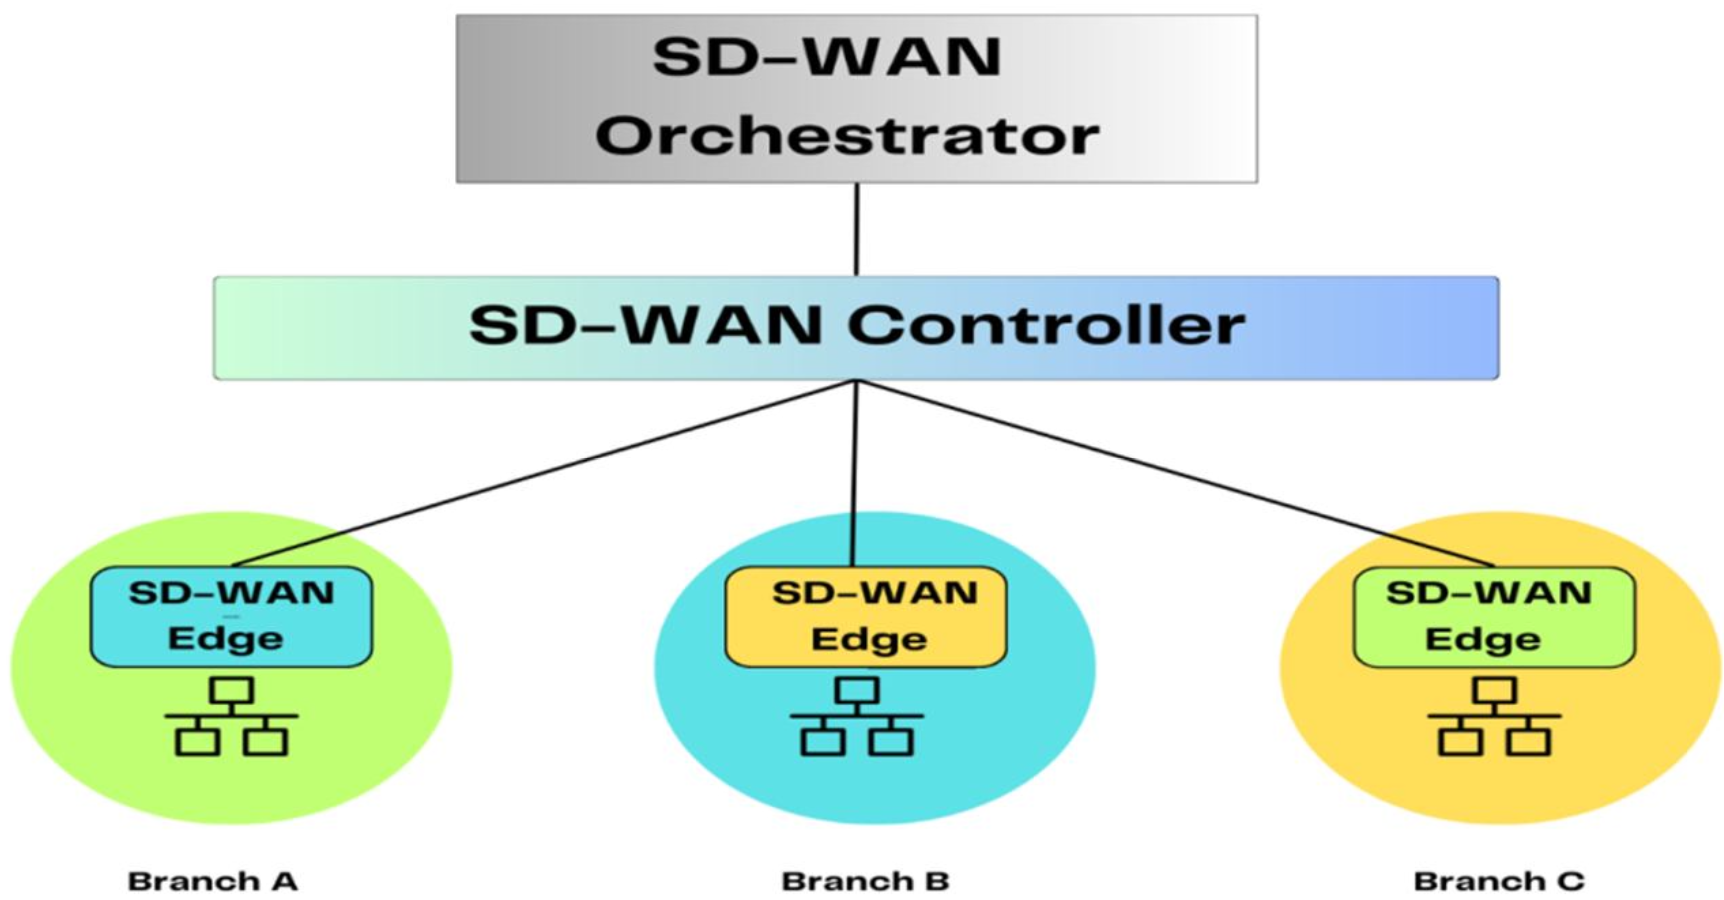
\includegraphics[width=\textwidth]{SD-WAN-architectuur.png}
  \caption[SD-WAN architectuur]{Software Defined WAN (SD-WAN)~\autocite{ijraset2025}}
  \label{fig:SD-WAN-architectuur}
\end{figure}

\subsection{Performantie}
In een onderzoek van arXiv~\autocite{arxiv2025} wordt de performantie van SD-WAN vergeleken met traditionele MPLS-netwerken. De onderzoekers voerden gecontroleerde experimenten uit om de routingfunctionaliteit en transmissie-efficiëntie te evalueren. Ze vergeleken de SD-WAN architectuur met de traditionele architectuur door ICMP-pakketten te versturen tussen verschillende locaties. Hoewel beide architecturen 100\% bereikbaarheid behaalden, vertoonde de SD-WAN architectuur hogere Round-Trip Time (RTT) waarden(Zie Figuur \ref{fig:SD-WAN-performance}). Deze verhoogde latentie wordt toegeschreven aan de multi-layer structuur van SD-WAN die meer dynamische dataflow mogelijk maakt maar ten koste van transmissievertraging.
\begin{figure}[H]
  \centering
  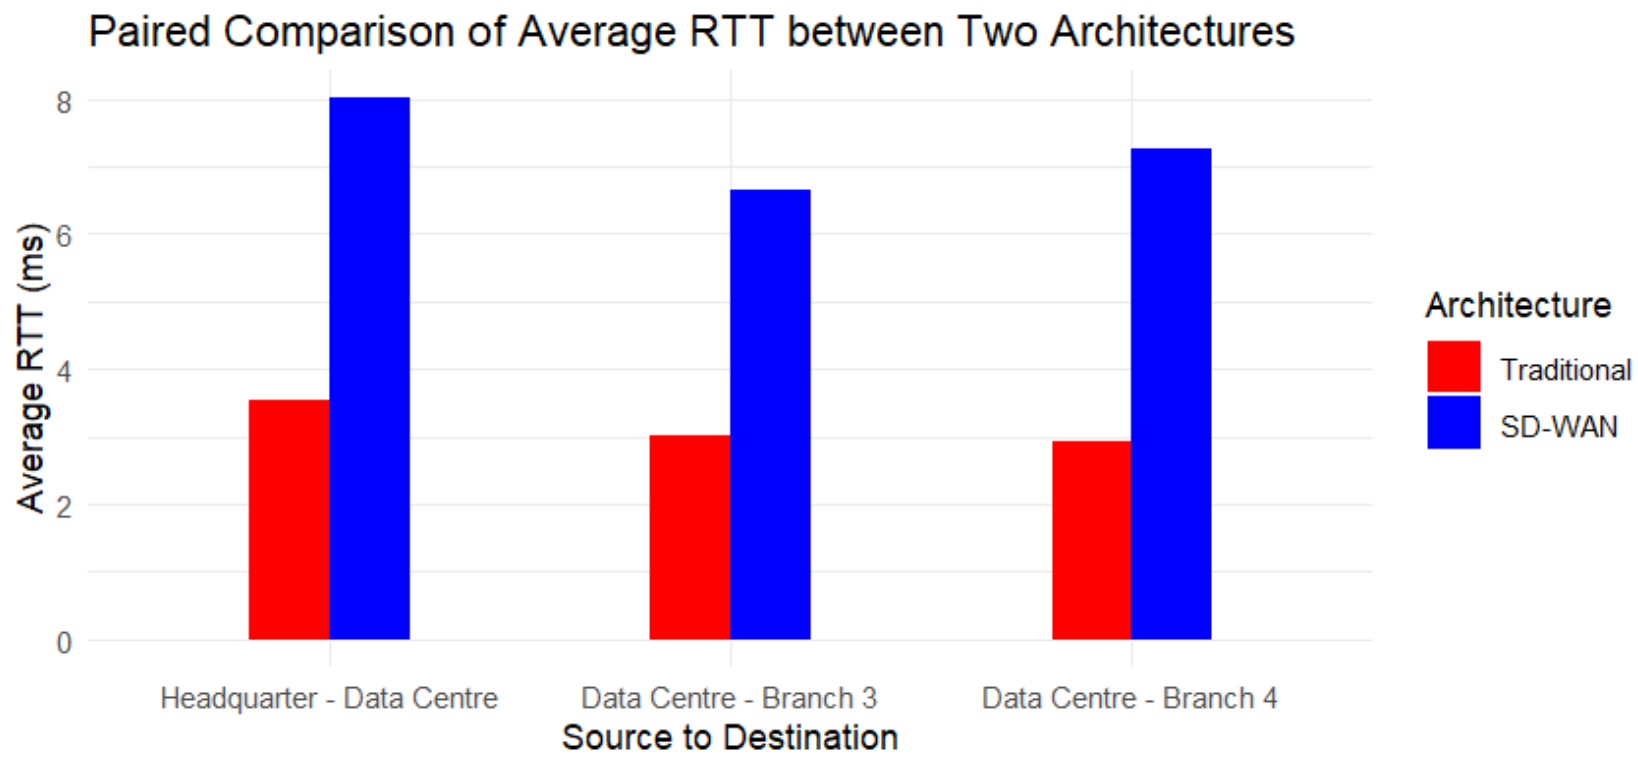
\includegraphics[width=\textwidth]{SD-WAN-performance.png}
  \caption[SD-WAN performantie]{Software Defined WAN (SD-WAN) performantie t.o.v. traditionele architectuur~\autocite{arxiv2025}}
  \label{fig:SD-WAN-performance}
\end{figure}

\subsection{De rol van SD-WAN in SASE}
SASE combineert verschillende services tot een samenhangende set van functies, waaronder threat protection, data leak prevention (DLP), DNS, Cloud Access Security Broker (CASB), Cloud Secure Web Gateway (SWG), Zero Trust Network Access (ZTNA), Web Application and API Protection as a Service (WAAPaaS), Firewall-as-a-Service (FWaaS) en Remote Browser Isolation (RBI). SD-WAN en SASE zijn bijzonder geschikt voor edge computing, waar low-latency services en real-time dataverwerking essentieel zijn voor applicaties zoals autonome voertuigen, healthcare monitoring en industriële automatisering~\autocite{ijraset2025}.